\documentclass{article}
\usepackage[utf8]{inputenc}
\usepackage{amsmath, graphicx}
\usepackage[]{algorithm2e}
\usepackage[margin=1in]{geometry}

\allowdisplaybreaks

\makeatletter
\renewcommand\thesection{}
\renewcommand\thesubsection{\@arabic\c@section.\@arabic\c@subsection}
\makeatother

\title{\vspace{-5ex}Random Graphs Project 4}
\author{Alex Rose, Pedro Rodriguez}
\date{April 2016}

\begin{document}

\maketitle
\vspace{-15ex}
\section{}
\subsection{ }
\vspace{-2ex}
$$P(E_n) = pP(E_{n-1}) + (1-p)P(\neg E_{n-1}) = pP(E_{n-1}) + (1-p)(1- P(E_{n-1}) $$
$$ = (2p-1)P(E_{n-1}) + (1 - p), P(E_0) = p$$
\vspace{-2ex}
\subsection{} 
\vspace{-2ex}
Let $f(x) = (2p -1)x + (1-p)$. Note that for any real $x_1,x_0$:
$$|f(x_1) - f(x_0)| = |(2p-1)x_1 + (1-p) - (2p-1)x_0 - (1-p)| = |(2p-1)(x_1-x_0)|$$
This quantity is strictly less than $|x_1-x_0|$ if $0 < p < 1$, so f(x) is a contraction on that interval. So by the Contraction Mapping Theorem, the recursion will converge to f(x)'s unique fixed point on $0 < p < 1$ .  Solving for this fixed point:
$$x = (2p-1)x + (1-p)$$
$$2x - 2px = 1-p$$
$$x = \frac{1-p}{2(1-p)} = 1/2$$

So $\lim_{n\to\infty} P(E_{n})= x = 1/2$
\vspace{-2ex}
\subsection{}
\vspace{-2ex}
Each step of the process removes 2 "degrees" from the degree list to form 1 edge. We have D degrees, so this process will form $D/2$ edges in total.
\vspace{-2ex}
\subsection{}
\vspace{-2ex}
With the first procedure, the probabilities of a degree being even are identical between all degrees. The second procedure generates an unrestricted $n-1$ sized degree list; each of these degrees will be even with exactly probability $p$, and their sum will be even with probability $1/2$ for large $n$. But the final restricted degree must match the parity of the unrestricted degrees' sum, so it'll be even with probability $1/2$ \textit{regardless of p}. So the probabilities of a degree being even are not neccesarily identical between all degrees, and thus the two procedures aren't equivalent.

$$
\begin{aligned}
P(E_{n-1})&=P(d_1+...d_{n-1}=even)=P(d_1+...d_{n-1}=odd)=\frac{1}{2}\\
P(d_1+...+d_n=even)&=P(d_n=even,d_1+...d_{n-1}=even)+P(d_n=odd,d_1+...d_{n-1}=odd)\\
&=P(d_n=even)P(d_1+...d_{n-1}=even)+P(d_n=odd)P(d_1+...d_{n-1}=odd)\\
&=\frac{1}{2}[P(d_n=even)+P(d_n=odd)]=\frac{1}{2}\cdot 1=\frac{1}{2}=P(E_n=even)
\end{aligned}
$$

Since the overall probability of getting an even event after fixing $d_{n-1}$ (whose even/oddness is itself random, but equal in probability) is $\frac{1}{2}$, that means the procedures are equivalent.

\vspace{-2ex}
\subsection{} 
\vspace{-2ex}
\begin{algorithm}[H]
 Degrees = None, Edges = NxN Matrix\;
 \While{Degrees is None}{
 Vec = create N length vector with N draws from simulate(d)\;
  \If{sum of Vec is even}{
	Degrees = Vec\;
   }
 }
half\_edges = create a list with Degrees[i] instances of i\;
random.shuffle(half\_edges)\;
\While{len(half\_edges) above 0}{
	u, v = pop(half\_edges), pop(half\_edges\;
	\If{u == v}{
	Edges[u, v] += 1
	}
	\Else{
	Edges[u,v] += 1
	Edges[v,u] += 1
	}
 }
\Return Edges

\end{algorithm}

\subsection{}
\vspace{-2ex}
Let $S_t = d_1 + d_2 + ... + d_t$. Then:

$$q_n  = \begin{cases}
  P(E_{n-t}), & \text{if } S \text{ is even}, \\
  1 - P(E_{n-t}), & \text{if }  S \text{ is odd}.
\end{cases}$$

As $t$ is finite, we have:
$$\lim_{n\to\infty} P(E_{n-t}) = \lim_{n\to\infty} P(E_{n})  = 1/2$$. 

So $\lim_{n\to\infty} q_n = 1/2$ in both cases.

\subsection{}
\vspace{-2ex}
Let $D_t$ denote event $(d_1 = k_1, d_2 = k_2,..., d_t = k_t)$. By Baye's Theorem:

$$ \lim_{n\to\infty} P(D_t | E_n) = \lim_{n\to\infty} \frac{P(E_n | D_t)P(D_t)}{P(E_n)} = \frac{1/2* P(D_t)}{1/2} = P(D_t) $$

And the variables $d_1...d_n$ are all independent by assumption, so:
$$P(D_t) = P(d_1 = k_1) P(d_2 = k_2) ... P(d_t = k_t) = \prod_{j=1}^{t} P(d_j)$$ 

\section{}
\subsection{}
$$
\begin{aligned}
&d\sim Binomial(n,p),n=5,p=1/2\\
\mu_1&=E[d]=np\\
E[d^2]&=Var(d)+E[d]^2=np(1-p)+n^2p^2=np-np^2+n^2p^2\\
\mu_2&=E[d^2]-E[d]=np-np^2+n^2p^2-np=n^2p^2-np^2\\
\frac{\mu_2}{2\mu_1}&=\frac{n^2p^2-np^2}{2np}=\frac{np-p}{2}=1=(\frac{\mu_2}{2\mu_1})^2
\end{aligned}
$$

$$
\begin{aligned}
&d\sim Geometric(p),p=2/5\\
\mu_1&=E[d]=\frac{1}{p}\\
E[d^2]&=Var(d)+E[d]^2=\frac{1-p}{p^2}+\frac{1}{p^2}\\
\mu_2&=E[d^2]-E[d]=\frac{1-p}{p^2}+\frac{1}{p^2}-\frac{1}{p}=\frac{2-2p}{p^2}\\
\frac{\mu_2}{2\mu_1}&=\frac{2-2p}{2p^2}\cdot p=\frac{1-p}{p}=1.5\\
(\frac{\mu_2}{2\mu_1})^2&=2.25
\end{aligned}
$$

For all experiments $n=250$

The results show that for the binomial we wish to compare against $Poisson(1)$ and geometric against $Poisson(1.5)$. Experimental results are shown in figure \ref{loop}. The plots agree well with theoretical results.

\begin{figure}[!ht]
	\centering
	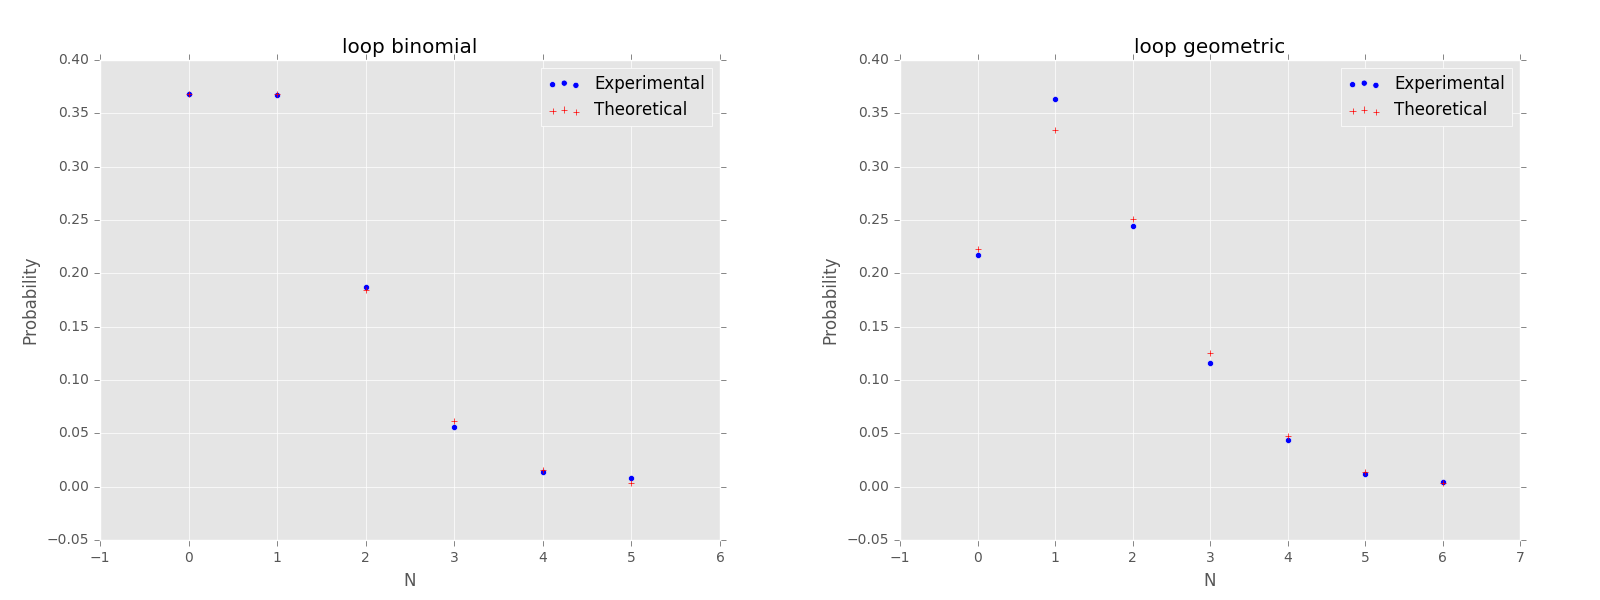
\includegraphics[width=\textwidth]{loop.png}
	\label{loop}
\end{figure}

\subsection{}
\vspace{-2ex}
The results show that for the binomial we wish to compare against $Poisson(1)$ and geometric against $Poisson(2.25)$. Experimental results are shown in figure \ref{parallel}. The plots agree well with theoretical results.

\begin{figure}[!ht]
	\centering
	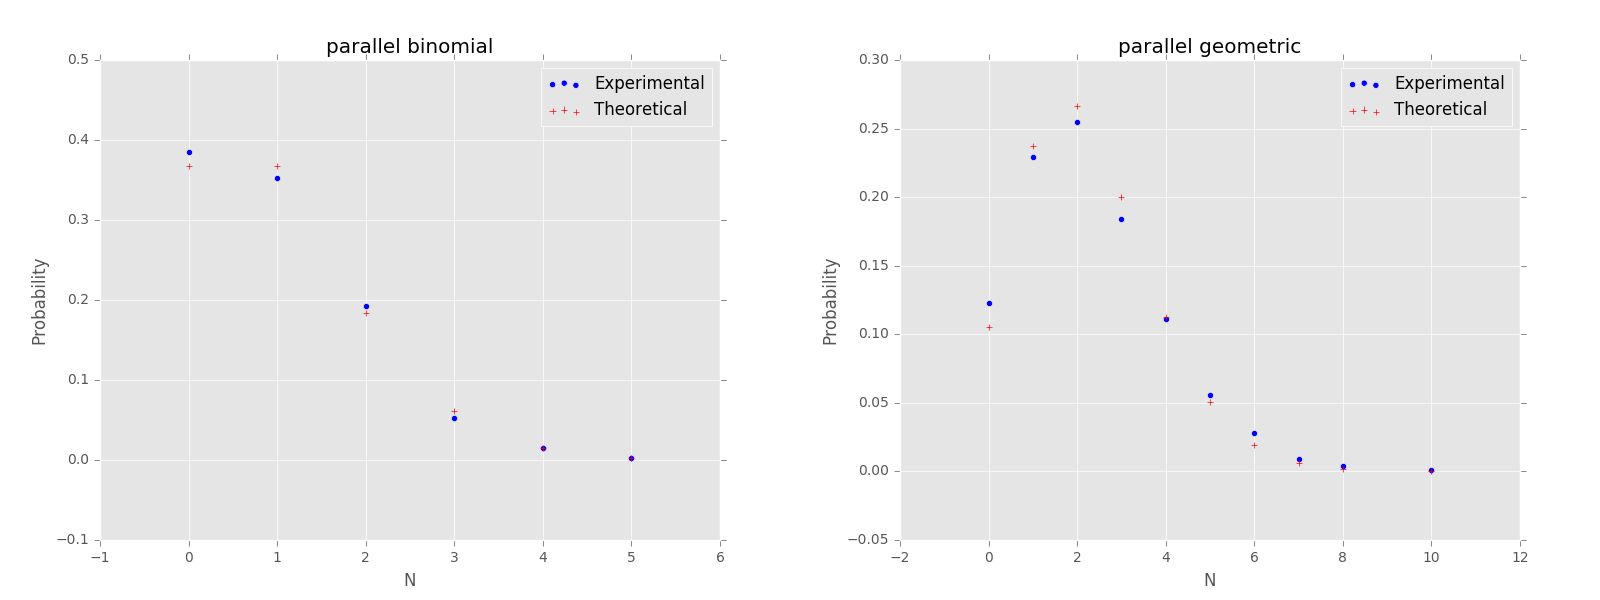
\includegraphics[width=\textwidth]{parallel.png}
	\label{parallel}
\end{figure}

\subsection{}
\vspace{-2ex}
The counts of loops and parallel edges in a simple graph is zero, thus:

For $d\sim Binomial(5,1/2)$, $P(simple)=p_1(0)\cdot p_1(0)=.367^2=.135$. Five experimental runs of 1K graphs yields $[.131,.12,.138,.118,.144]$ which agrees well with the theoretical result.

For $d\sim Geometric(2/5)$, $P(simple)=p_{1.5}(0)\cdot p_{2.25}(0)=.0235$. Five experimental runs of 1K graphs yields $[.03,.026,.03, .025, .023]$. These results generally agre, but not that the mean of the runs is slightly high. To alleviate this, a higher $n$ may help, but was difficult because counting parallel edges in our algorithm is $O(n^2)$ and took a long time to ran for anything significantly above $n=250$.

\end{document}
